\documentclass[t,12pt]{beamer}

\usepackage[T1]{fontenc} 
\usepackage[frenchb]{babel}
\usepackage[utf8]{inputenc}

\usetheme{Berkeley}
\usecolortheme{dove}

\title{Notes export from an Ebook Sony PRS-T1}
\author{Tutor: Julien De Antoni\\Grégory Putz, Ahma Bekele, Mathieu Bivert}
\date{\oldstylenums{June 2012}}
% ajouter tuteur
% rajouter plan continu
% intro
% annonce du plan
% analyse du sujet
% resultats
% problèmes & évolution

\begin{document}
\frame{\titlepage}

\section{Introduction}

\begin{frame}
  \frametitle{Introduction}
  some more introductive text
\end{frame}

\begin{frame}
  \frametitle{Introduction}
  \centering
  \tableofcontents
\end{frame}

% \begin{frame}
% $\vcenter{
% \begin{figure}[!ht]
%   \vfill
%   \centering
%   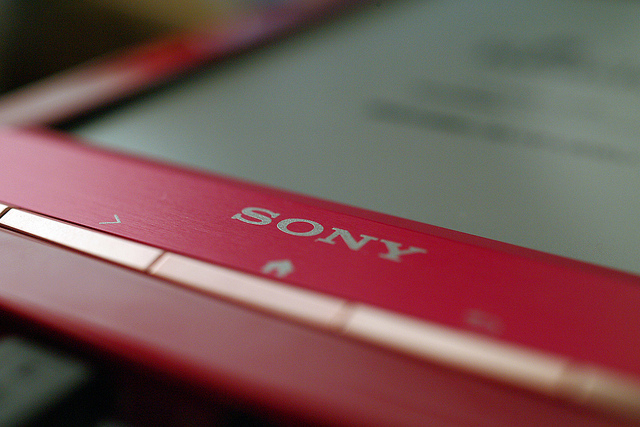
\includegraphics[scale=1]{prs-t1.png}
% \end{figure}}$
% \end{frame}

% \begin{frame}
%   \frametitle{An Ebook-reader}
%   Advantages of a reader over a bookcase:
%   \begin{itemize}
%     \pause \item portable, light;
%     \pause \item economical/ecological (nowadays, paper is mainly manufactured from trees…);
%     \pause \item non-destructive note taking;
%     \pause \item files and notes sharing;
%     \item etc.
%   \end{itemize}
%   \pause Notably usefull for researchers, avid readers, etc.
% \end{frame}

\section{Specifications}
\begin{frame}
  \frametitle{Specifications}
  \begin{itemize}
  \pause \item Sharing notes;
  \pause \item No standardized note taking format.
  \pause \item Notes stored on the ebook:
    \begin{itemize}
      \item half in SQLite;
      \item half in XML (SVG).
    \end{itemize}
  \pause In a nearly comprehensible format.
  \end{itemize}
\end{frame}

\begin{frame}
  \frametitle{Specifications : client requests}
  \begin{itemize}
    \item GNU/Linux,
    \pause Sony software is closed source, windows only (although
    it may run on wine), and not supporting cut2col (used by the
    client);
    \pause \item main task : export PDF with notes; \pause others :
    import PDF, manage Epub, etc.
  \end{itemize}
\end{frame}

\begin{frame}
  \frametitle{Specifications: existing work}
  Calibre : software to import/export ebook to a reader\\
  $\rightarrow$ create a plugin for calibre in Python,\\
  \pause while trying software notes format (xournal, okular),
  found PDF has annotations\\
  \pause some Java APIs found to manage PDF.
\end{frame}

\section{Organisation}
\begin{frame}
  \frametitle{Task assignments}
  Separation in 3 parts :
  \begin{itemize}
    \pause \item data recovery and treatment
	\pause \item exportation of annotation
	\pause \item user interface
  \end{itemize}
\end{frame}

\begin{frame}
  \frametitle{Task assignments}
  \begin{itemize}
    \pause \item database :
	\begin{itemize}
		\item study of database architecture
		\item extraction of necessary information
		\item permanent communication to target the needs
	\end{itemize}
	\pause \item exportation :
	\begin{itemize}
		\item study of storage format of the annotations
		\item parsing of the XML files
		\item insert annotations in PDF file
	\end{itemize}
	\pause \item ui :
	\begin{itemize}
		\item MVC pattern
		\item graphical interface
		\item console interface
	\end{itemize}
  \end{itemize}
\end{frame}

\section{A solution}
\begin{frame}
  \frametitle{A solution}
  \begin{itemize}
    \item in Java (portability) and ease of developpment (pre-existing
      librairies, etc.);
    \pause \item with iText for PDF manipulation (free, open);
    \pause \item console and graphical (SWT, portability) interfaces;
  \end{itemize}
\end{frame}

\section{Encountered problems}
\begin{frame}
  \frametitle{Encountered problems}
  We don't neeeeed, no more problems.
\end{frame}

\section{To conclude}
\begin{frame}
	\frametitle{Outcome}
	As planned, we succeeded in :
	\begin{itemize}
		\pause \item exporting notes from Ebook to PC
		\pause \item making a portable application
		\pause \item offering a friendly user interface
	\end{itemize}
	Possible extensions :
	\begin{itemize}
		\pause \item import notes from PC to Ebook
		\pause \item manage others formats than PDF
		\pause \item put keyboard notes in the right place in the text
	\end{itemize}
\end{frame}

\begin{frame}
  \frametitle{Outcome}
  \begin{itemize}
    \item Technical point of view :
	\begin{itemize}
		\item implementation of different skills
		\item internal functioning of an Ebook
		\item use of database
		\item use of some Java libraries
		\item data translation between different formats
	\end{itemize}
	\pause \item Personal point of view :
	\begin{itemize}
		\item improve the skills in team working
		\item realize a soft that could be used in the future
		\item give a presentation in English
	\end{itemize}
  \end{itemize}
\end{frame}

\begin{frame}
  \frametitle{Demonstration!}
  $\vcenter{
    \begin{figure}[!ht]
      \vfill
      \centering
      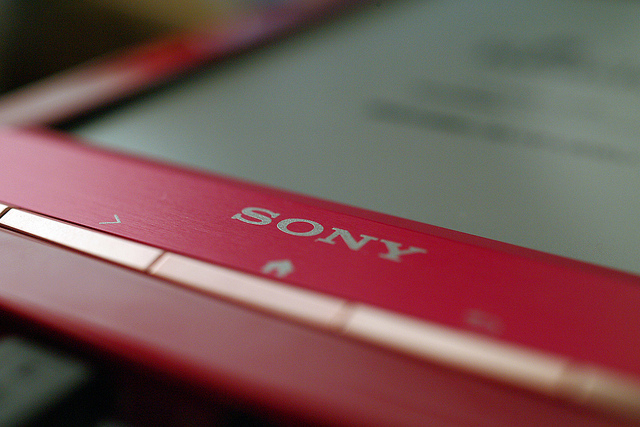
\includegraphics[scale=1]{prs-t1.png}
  \end{figure}}$
\end{frame}

\end{document}
